\chapter{Experiments}
\label{cha:experiments}

The previous chapter showed how much faster the CUDA implementation is compared to the same algorithm implemented on the CPU. This significant increase in performance allows for new experiments.

We will now perform a number of experiments to explore the numerical precision and validate the results against prior research. We begin by looking at tumbling orbits, a very delicate experiment requiring great precision. This is followed by a quick look at the effect of the fiber concentration on the required GMRES iterations to settle on the solution. Next we reproduce a very interesting physical phenomenon of letting a sphere of fibers sediment and validate our results against similar experiment by others. Furthermore, we will have a brief exploration of the effects of the number of fibers and the concentration of fibers on the sphere simulation. All experiments were run with the purely numerical, 2-dimensional CUDA algorithm  implemented in the thesis. The systems were solved using the direct solver from MAGMA in order to avoid variations in the run time.

\section{Tumbling orbits}
\label{sec:example_ring}

The first example was used to verify that the single precision GPU version is able to replicate the result of the original double precision code. For this we looked at a very simple problem where a small number of fibers are set up with perfectly symmetrical positions and orientations. All fibers are evenly distributed on a circle and aligned vertically with gravity. During the simulation the fibers begin to rotate from their vertical orientation towards the horizontal position. Afterwards, they continue rotating back into the vertical position. This motion is referred to as tumbling orbits and as long as there are no disturbances or numerical precision issues it repeat forever.

This simple but very interesting problem has also been simulated by Gustavsson and Tornberg~\cite{Gustavsson2009}. Additionally an even more simplified version with only two fibers was studied both numerically and experimentally by Jung et al.~\cite{Jung2006}. This example is thus ideally suited to test and verify the numerical precision of the GPU simulation. A visualization of the GPU simulation of $16$ fibers evenly distributed around a circle with a radius of $0.55$, is shown in Fig.~\ref{fig:ring_simulation}.

\begin{figure}[!htbp]
  \centering
  \begin{subfigure}[h]{0.45\textwidth}
    \centering
    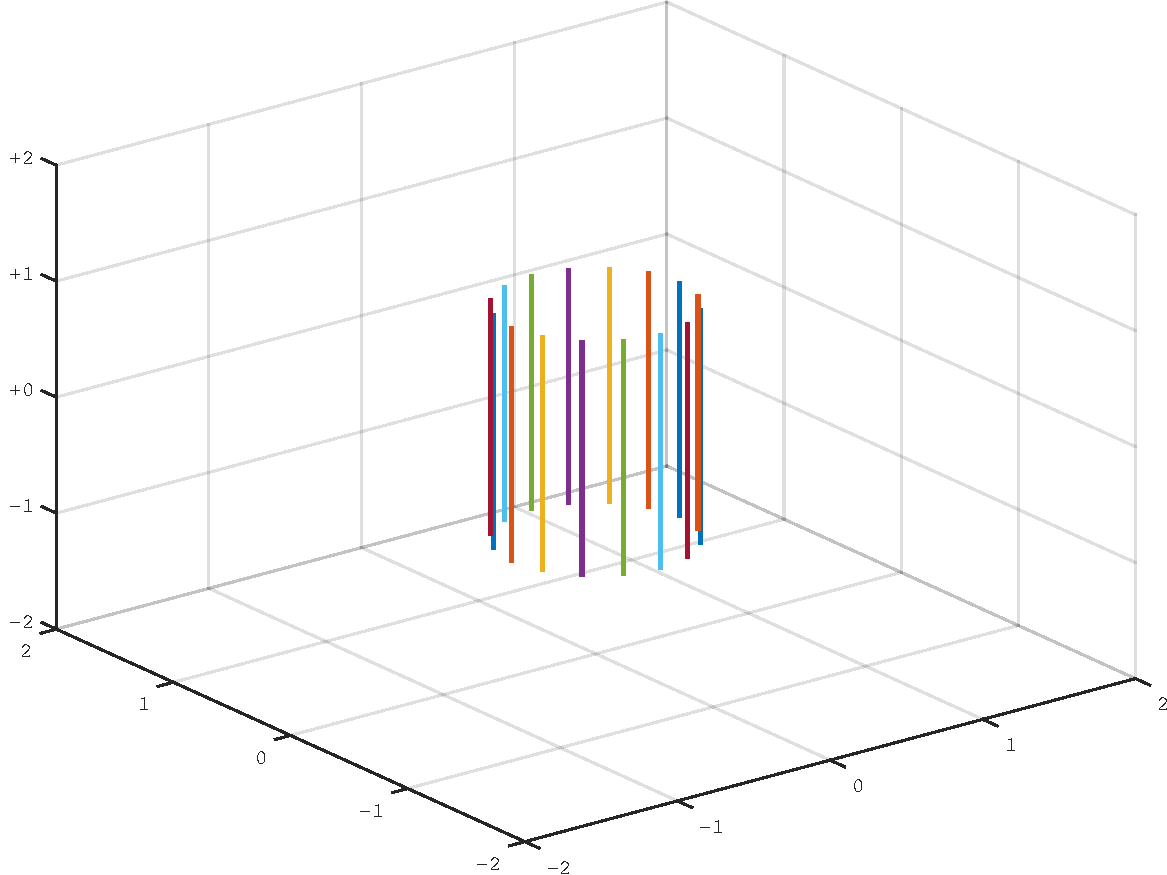
\includegraphics[width=\textwidth]{img/ring_00000.pdf}
    \caption{$t=0$}\label{fig:ring_simulation_1a}
  \end{subfigure}
  \begin{subfigure}[h]{0.45\textwidth}
    \centering
    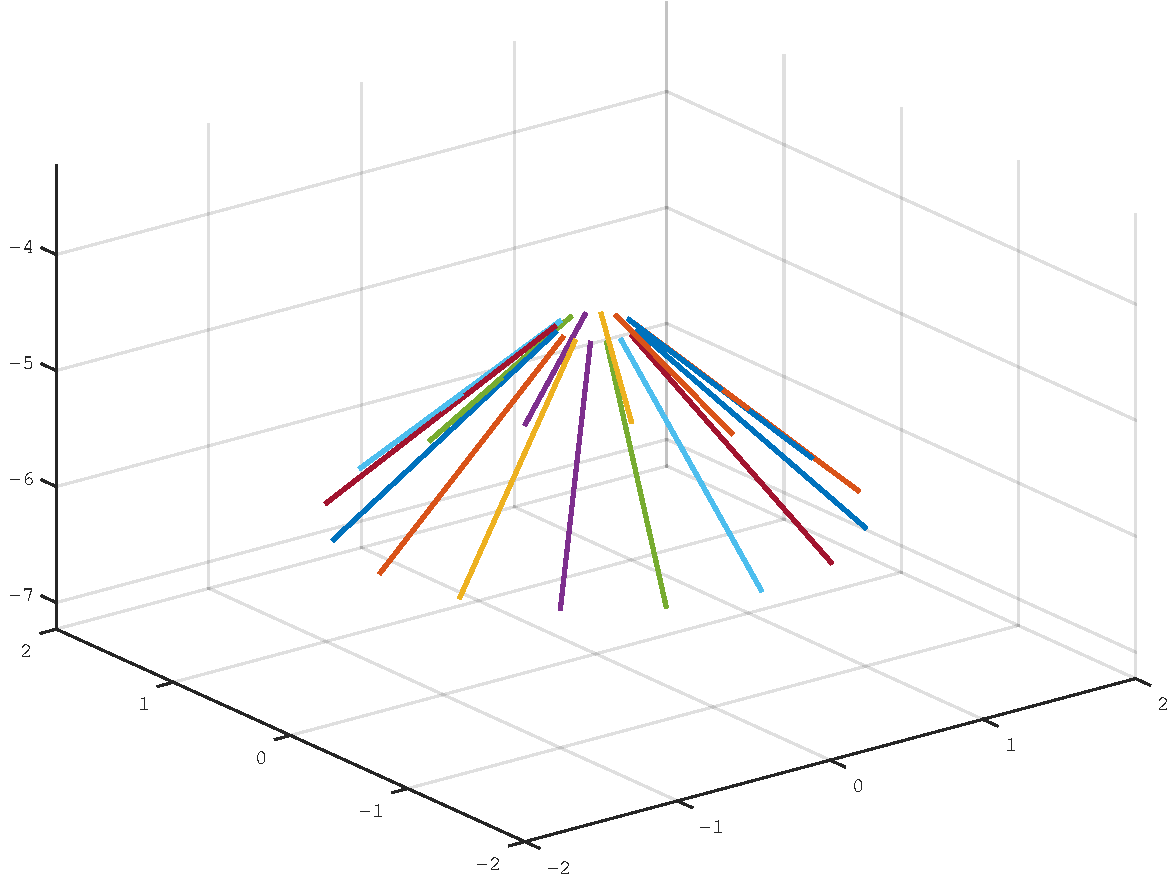
\includegraphics[width=\textwidth]{img/ring_00015.pdf}
    \caption{$t=15$}\label{fig:ring_simulation_1b}
  \end{subfigure}
  \begin{subfigure}[h]{0.45\textwidth}
    \centering
    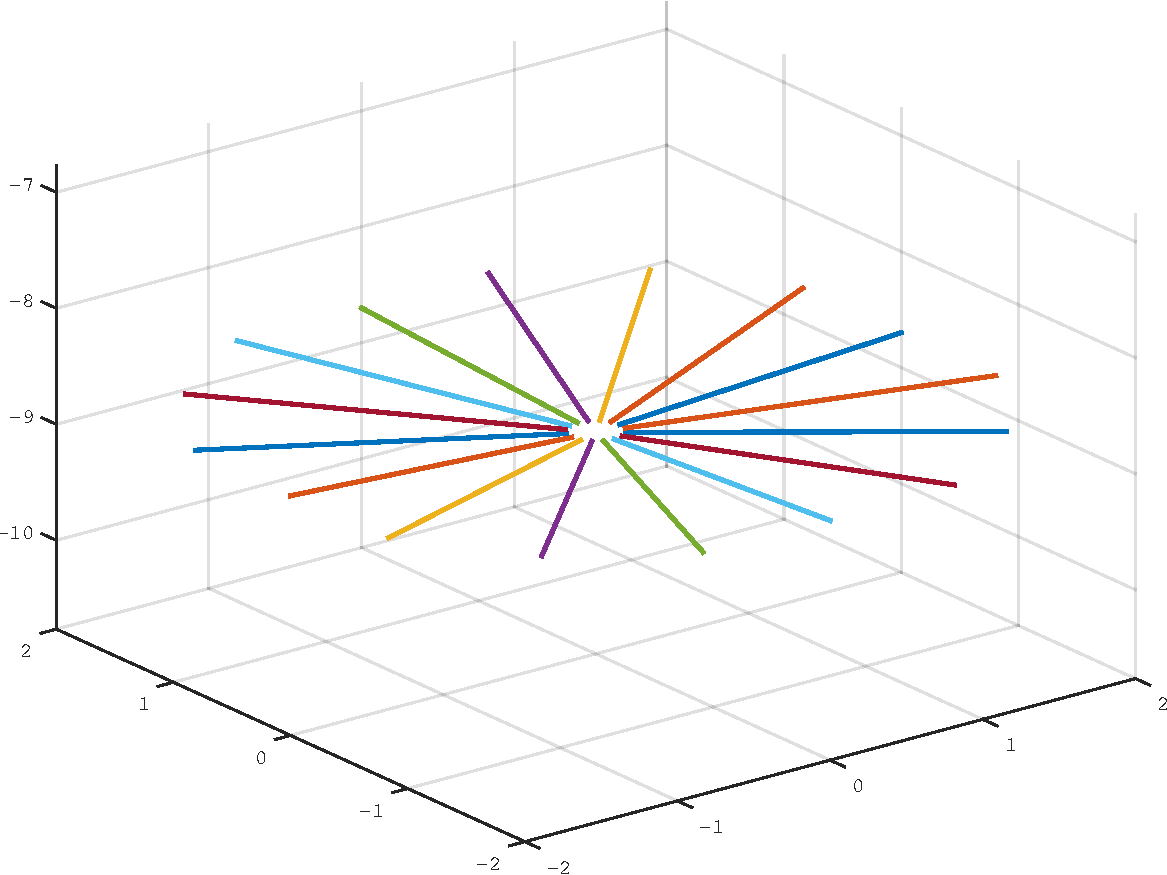
\includegraphics[width=\textwidth]{img/ring_00030.pdf}
    \caption{$t=30$}\label{fig:ring_simulation_1c}
  \end{subfigure}
  \begin{subfigure}[h]{0.45\textwidth}
    \centering
    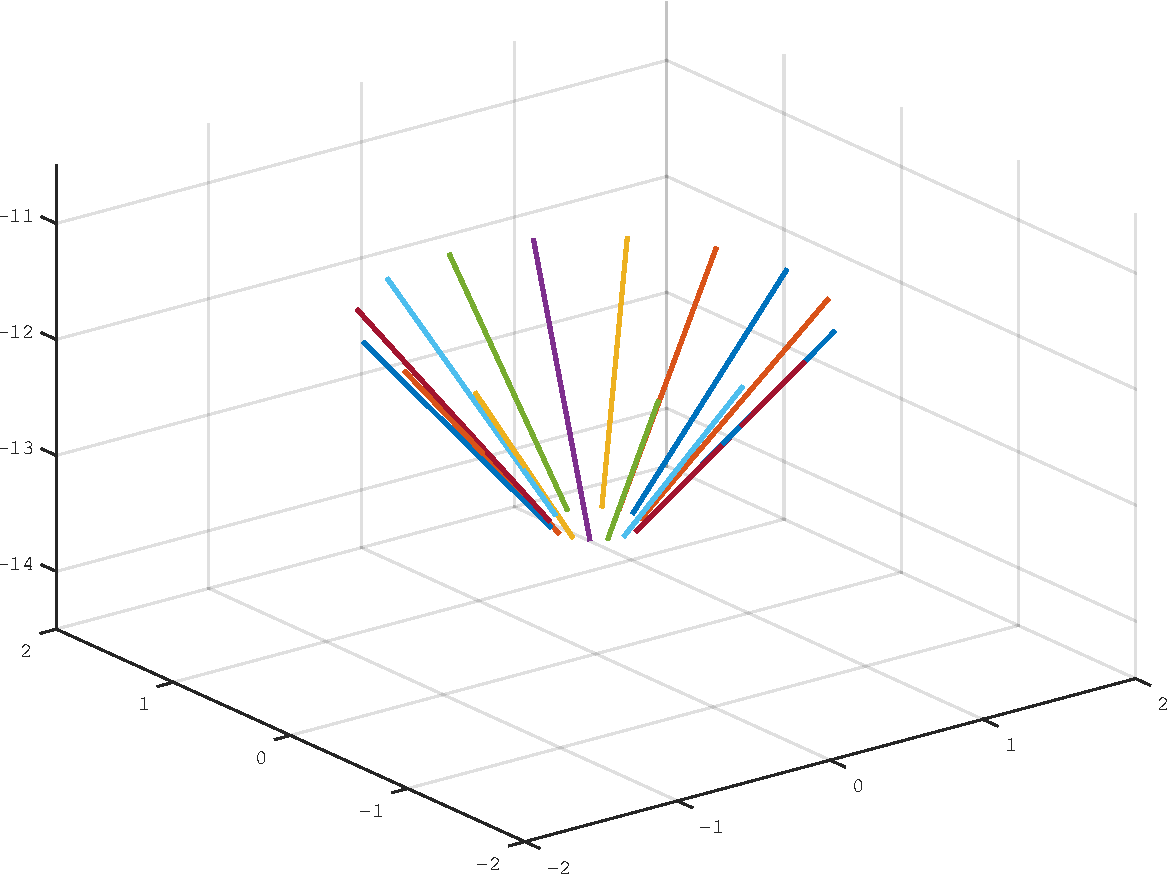
\includegraphics[width=\textwidth]{img/ring_00045.pdf}
    \caption{$t=45$}\label{fig:ring_simulation_1d}
  \end{subfigure}
  \caption[Visualization of tumbling orbits.]{Visualization of tumbling orbits. Small number of perfectly symmetrically distributed fibers around a circle are allowed to sediment due to gravity. The fibers perform a periodical motion alternating between a vertical and horizontal orientation in the direction to gravity.}
  \label{fig:ring_simulation}
\end{figure}

In order to analyze the periodic movement of the fibers we now look at the sedimentation velocity caused by gravity. In the initial setup the fibers are aligned vertically and are dropping with the maximum velocity. As they rotate into the horizontal orientation the velocity is decreasing and reaches its minimum once the fibers are perpendicular to the direction of gravity. Afterwards on their way back to vertical orientation the velocity increases again.

Fig.~\ref{fig:ring_sedimentation_velocity} shows a graph of the sedimentation velocity of a single fiber over time for both the single precision GPU code and the original double precision Fortran code. As the same force acts on all fibers and they perform the same motion they all have the same sedimentation velocity. For this particular setup the maximum velocity is $~3.8$ and the minimum velocity is $~2.2$. The graphs clearly shows the periodical rotation the fiber perform. This result perfectly captures the expected result obtained from prior simulation and experiments.

\begin{figure}[!htbp]
  \centering
  \begin{tikzpicture}
    \begin{axis}[
      xlabel={Timestep},
      ylabel={Velocity},
      height={207pt},
      unbounded coords=discard,
      xmin=0,xmax=200,
      ymin=-4,ymax=-2,
      ]

      \addplot[color=set12, very thick] table[x=Timestep,y=Single] {charts/ring_sedimentation.csv};
      \addplot[color=set11, loosely dashed, ultra thick] table[x=Timestep,y=Double] {charts/ring_sedimentation.csv};
    \end{axis}
  \end{tikzpicture}
  \caption[Comparison of sedimentation velocity for single- and double-precision simulation.]{Comparison of sedimentation velocity for single precision (solid line) and double precision (dahsed line) simulation.}
  \label{fig:ring_sedimentation_velocity}
\end{figure}

\section{Fiber concentration effect on GMRES iterations}
\label{sec:example_concentration_gmres}

As alluded to in the discussion about the performance of direct solvers versus iterative solvers in Sec.~\ref{sec:bench_linear_solvers} we will now investigate how the concentration of fibers affects the GMRES iterations. In this context the concentration of fibers refers to the average distance between each fiber and its closest neighbor. Thus we use the average minimal pair-wise distance between the fibers as a measurement of fiber concentration. Fig.~\ref{fig:concentration_gmres} illustrates the number of iterations GMRS needs to solve the system for a given pair-wise distance. Please note that the x-axis as well as the y-axis are logarithmic to improve clarity.

\begin{figure}[!htbp]
  \centering
  \begin{tikzpicture}
    \begin{axis}[
      xlabel={Average distance},
      ylabel={GMRES iterations},
      width={0.8\textwidth},
      unbounded coords=discard,
      xmode=log,
      ymode=log,
      grid=major,
      xmin=0,xmax=100,
      ymin=0,ymax=400,
      ]

      \addplot[color=set11, mark=*,mark options={fill=white}, very thick] table[x=Concentration,y=Average] {charts/concentration_gmres.csv};

    \end{axis}
  \end{tikzpicture}
  \caption[Effect of fiber concentration on GMRES iterations.]{Effect of fiber concentration on GMRES iterations. The number of GMRES iterations increases dramatically for close fibers.}
  \label{fig:concentration_gmres}
\end{figure}

We can see that for an increasing average pair-wise distance, i.e. a lower fiber concentration, the number of iterations decreases. The average iteration count for the concentration (average distance of $0.4$) we used during our benchmarks in Chapter~\ref{cha:benchmarks} lies between $3$ and $10$. However, as the average pair-wise distance decreases we observe an exponential increase in the number of iterations.

To find the reason for this we have again have to look at the integral in Eqn.~\eqref{eq:inner_integral} which has to be solved for each fiber pair during the \emph{Assemble System} step. The required Stokeslet computations in Eqn.~\eqref{eq:stokeslet_stokeslet} include the distance between the fibers in the denominator. As the distance gets very small the value of the Stokeslet becomes large. These large terms can then cause the assembled matrix to become ill-conditioned and thus increase the number of iterations GMRES requires to settle on a solution.

This result is important to keep in mind when simulating long running complex fiber configuration. Here the probability that any two fibers get close to each other is very high. If this is the case solving the system using GMRES takes longer than expected. In practice it might thus be beneficial to switch to the direct solver, as it has a predictable runtime. This is especially true because the performance difference between direct and iterative solvers on the GPU is relatively small.

\section{Sedimenting sphere}
\label{sec:example_sphere}

The next example showcases a more chaotic system with a large number of interacting fibers. This experiment is studied by several papers, e.g.~\cite{Metzger2007}\cite{Park2010}\cite{Bulow2015}. It is especially interesting because the observed results only occur if enough fibers are simulated. Our GPU simulation is able to efficiently handle up to $2000$ fibers and is thus ideally suited for studying this example. For the experiment $2000$ fibers are initially distributed inside a sphere with a concentration of $0.4$. Both their positions and orientations are randomly generated inside this sphere. An illustration of an example run can be seen in Fig.~\ref{fig:sphere_simulation}.

\begin{figure}[!htbp]
  \centering
  \begin{subfigure}[h]{0.4\textwidth}
    \centering
    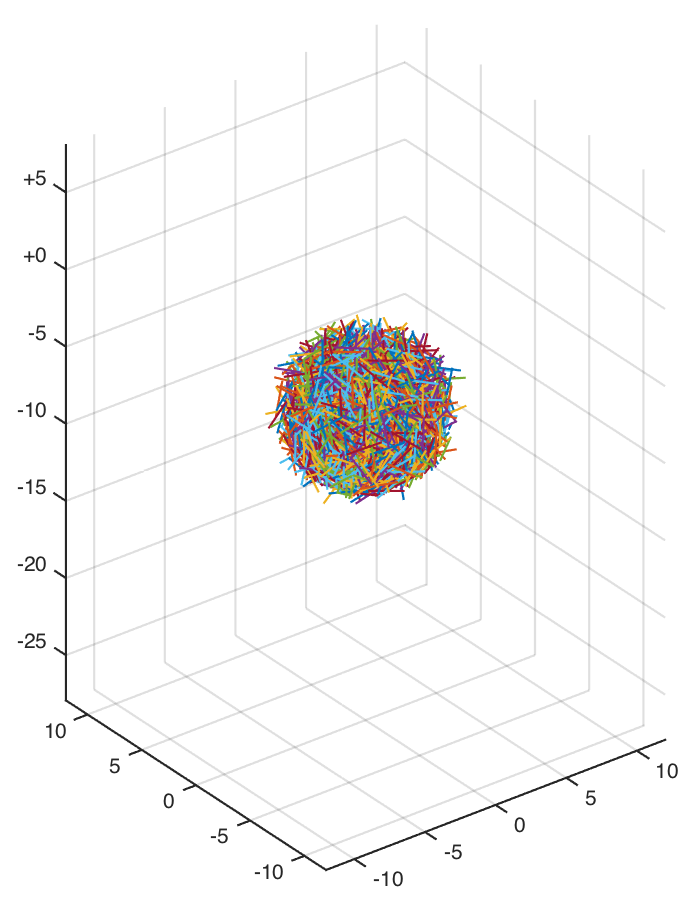
\includegraphics[width=\textwidth]{img/state_00000.pdf}
    \caption{$t=0$}\label{fig:sphere_simulation_1a}
  \end{subfigure}
  \begin{subfigure}[h]{0.4\textwidth}
    \centering
    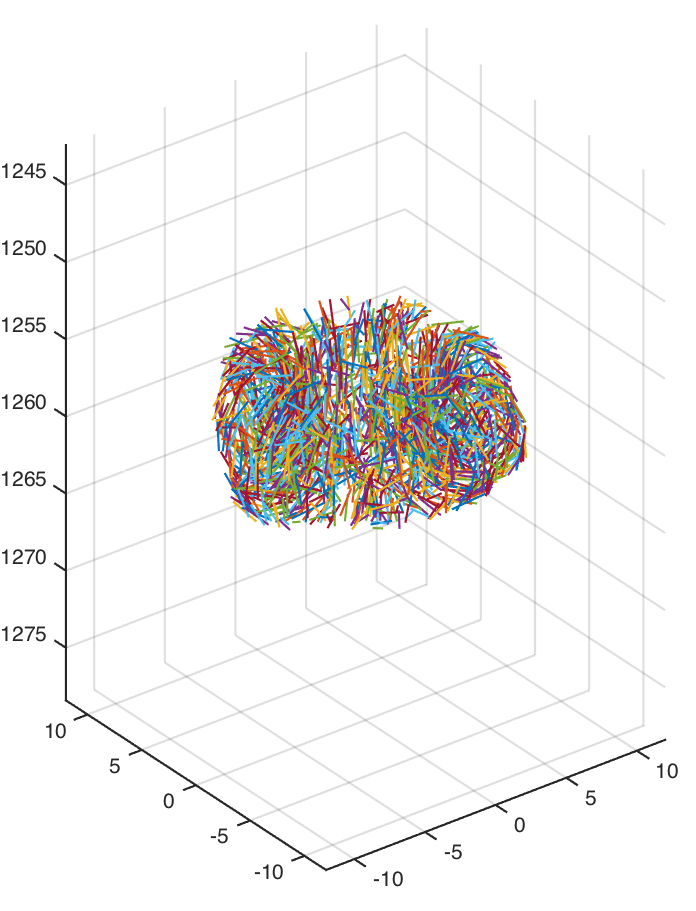
\includegraphics[width=\textwidth]{img/state_00250.pdf}
    \caption{$t=300$}\label{fig:sphere_simulation_1b}
  \end{subfigure}
  \begin{subfigure}[h]{0.4\textwidth}
    \centering
    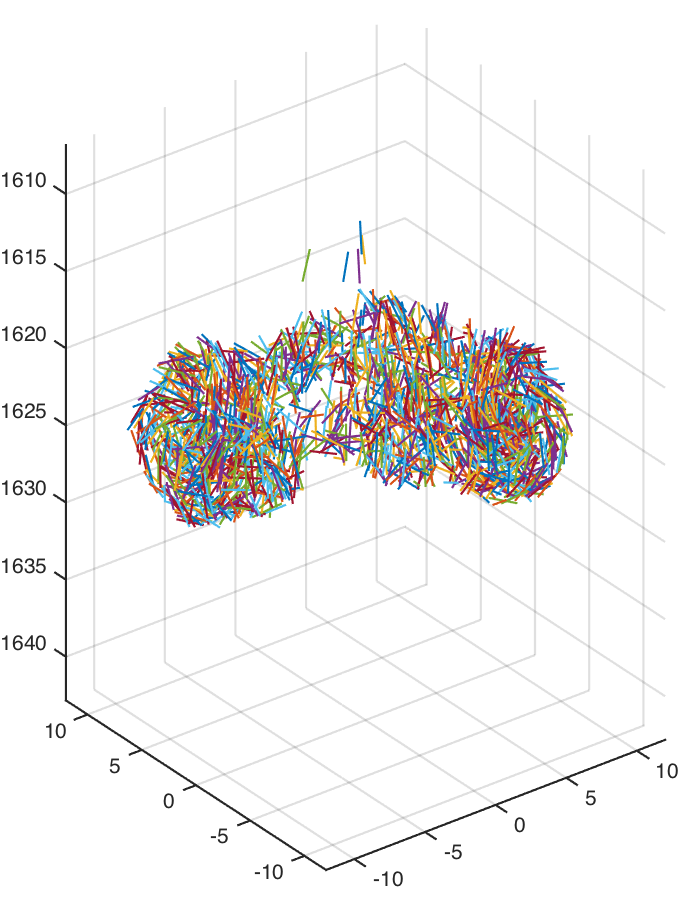
\includegraphics[width=\textwidth]{img/state_00350.pdf}
    \caption{$t=350$}\label{fig:sphere_simulation_1c}
  \end{subfigure}
  \begin{subfigure}[h]{0.4\textwidth}
    \centering
    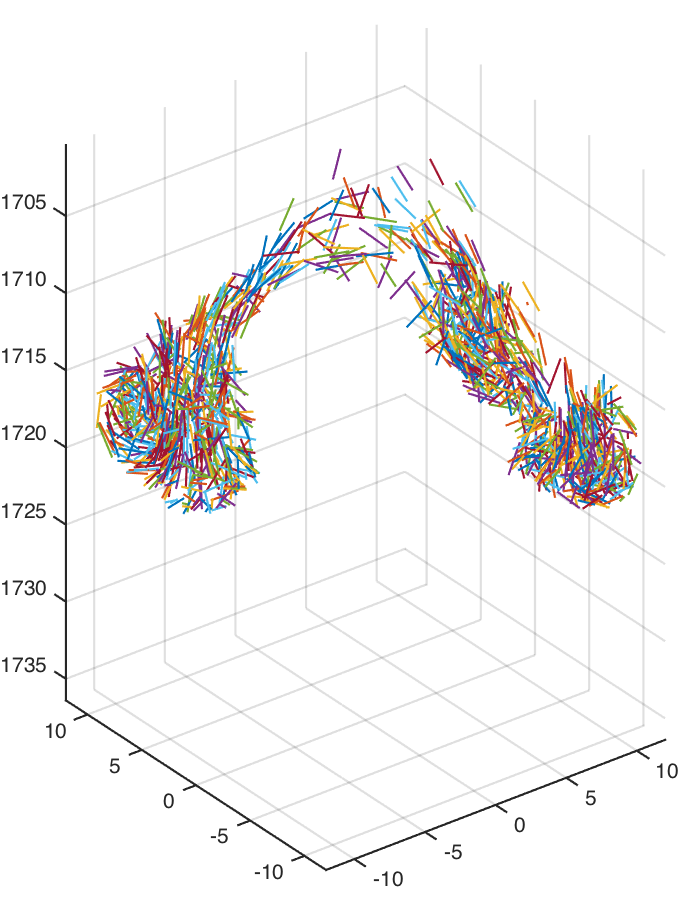
\includegraphics[width=\textwidth]{img/state_00380.pdf}
    \caption{$t=380$}\label{fig:sphere_simulation_1d}
  \end{subfigure}
  \caption[Visualization of sedimenting sphere.]{Visualization of sedimenting sphere. Fibers are randomly distributed inside a sphere and sediment due to gravity. The fibers proceed to form a turning torus. Eventually the torus breaks up into subclusters.}
  \label{fig:sphere_simulation}
\end{figure}

This sphere of packed fibers is then allowed to sediment due to gravity. Beginning from the spherical shape the interacting fibers slowly begin to form a continuously turning torus. Even though the behavior is more chaotic due to the large number of fibers and the random initial setup, this turning torus resembles the result for the tumbling orbits in Sec.~\ref{sec:example_ring}.

After some time the torus breaks and the fibers are split into multiple smaller clusters. Each cluster continues to sediment separately and slowly forms its own smaller torus again. However, due to tiny variations these toruses can be harder to see.

The calculation of the presented example only takes $~7.7$ seconds with the GPU simulation. Consequently it is possible to perform the $500$ time steps of the simulation in a little bit over $1$ hour. Simulating this many fibers in such a short time will allow new research of this interesting phenomenon. One interesting research question is for example determining what influences the stability of the torus.

\subsection{Sphere break-up}
To begin investigating this question we first define the stability of the torus in terms of the break up time. How to determine the exact break up time of the torus is quite challenging. This problem and question was also examined by Park et al.~\cite{Park2010}. They define the break up as the moment when the torus starts to bend prior to actually breaking. Additionally, they describe an algorithm that determines which fibers are part of the torus. Consequently, they compute metrics such as the remaining fibers, the radius and velocity of the sedimenting torus. Unfortunately, they don't define a metric that determines the exact break up time. Thus we came up with our own measure of the break up time based on their work.

We use the same definition for the torus as described by Park et al.~\cite{Park2010}. First we compute the initial horizontal radius $R_0$ of the sphere. Then as the sphere sediments and starts forming the torus a small number of fibers are separate. For each time step the center of mass of all fibers belonging to the torus is calculated. Any fibers with a distance larger than $R_0$ in the direction of gravity are excluded from the active set of fibers belonging to the torus. For the remaining fibers we then calculate the radius $R$ of the torus in each horizontal direction and the mean sedimentation velocity $V_z$. The torus metrics are illustrated for a sample run with $2000$ fibers and an average distance of $0.4$ in Fig.~\ref{fig:torus}. The horizontal radii $R_x$ and $R_y$ of the torus and the percentage of fibers remaining in the torus are shown in Fig.~\ref{fig:torus_radius} and Fig.~\ref{fig:torus_fibers}. The curves show the expected loss of fibers and the increasing torus radius.

\begin{figure}[!htbp]
  \centering
  \begin{subfigure}[h]{.48\textwidth}
	  \begin{tikzpicture}
	    \begin{axis}[
	      xlabel={Timestep},
	      ylabel={Radius},
	      width={\textwidth},
	      unbounded coords=discard,
	      xmin=0,xmax=500,
	      grid=major,
	      every axis label/.append style={font=\sffamily\footnotesize},
	      ]
	
	      \addplot[color=set11, very thick] table[x=Timestep,y=RadiusX,col sep=comma] {charts/sphere_2000_0040.csv};
	      \addplot[color=set12, very thick] table[x=Timestep,y=RadiusY,col sep=comma] {charts/sphere_2000_0040.csv};
	
	      \legend{$R_x$,$R_y$}
	    \end{axis}
	  \end{tikzpicture}
    \caption{Torus radius.}\label{fig:torus_radius}
  \end{subfigure}
  \begin{subfigure}[h]{.48\textwidth}
	  \begin{tikzpicture}
	    \begin{axis}[
	      xlabel={Timestep},
	      ylabel={Fibers in torus (\%)},
	      width={\textwidth},
	      unbounded coords=discard,
	      xmin=0,xmax=500,
	      ymin=0.9,ymax=1.0,
	      grid=major,
	      legend pos=north east,
	      every axis label/.append style={font=\sffamily\footnotesize},
	      ]
	
	      \addplot[color=set11, very thick] table[x=Timestep,y=NormalizedN,col sep=comma] {charts/sphere_2000_0040.csv};
	
	      \legend{$M / M_0$}
	
	    \end{axis}
	  \end{tikzpicture}
    \caption{Remaining fibers.}\label{fig:torus_fibers}
  \end{subfigure}
  \begin{subfigure}[h]{.48\textwidth}
	  \begin{tikzpicture}
	    \begin{axis}[
	      xlabel={Timestep},
	      ylabel={Radius},
	      width={\textwidth},
	      unbounded coords=discard,
	      xmin=0,xmax=500,
	      grid=major,
	      every axis label/.append style={font=\sffamily\footnotesize},
	      ]
	
	      \addplot[color=set12, mark=*,mark options={fill=white}, very thick] table[x=Timestep,y=RadiusZStd,col sep=comma] {charts/sphere_2000_0040_highlight.csv}
	node[pos=444, pin={[pin edge={color=set12, very thick}]min}]{};
	\addlegendentry{}
	      \addplot[color=set11, very thick] table[x=Timestep,y=RadiusZStd,col sep=comma] {charts/sphere_2000_0040.csv};
		\legend{,$R_z^{\text{std}}$};
	    \end{axis}
	  \end{tikzpicture}
    \caption{Torus $\text{Radius}_z$ Deviation.}\label{fig:torus_deviation}
  \end{subfigure}
  \begin{subfigure}[h]{.48\textwidth}
	  \begin{tikzpicture}
	    \begin{axis}[
	      xlabel={timestep},
	      ylabel={fibers in torus},
	      width={\textwidth},
	      unbounded coords=discard,
	      xmin=0,xmax=500,
	      grid=major,
	      legend pos=north east,
	      every axis label/.append style={font=\sffamily\footnotesize},
	      ]
	
	      \addplot[color=set11, very thick] table[x=Timestep,y=VelocityZ,col sep=comma] {charts/sphere_2000_0040.csv};
	
	      \legend{$V_z$}
	
	    \end{axis}
	  \end{tikzpicture}
    \caption{Mean sedimentation velocity.}\label{fig:torus_velocity}
  \end{subfigure}
  \caption[Evolution of the sedimenting torus.]{Evolution of the sedimenting torus. In the beginning the torus loses some fibers and the horizontal radii $R_x$ and $R_y$ increase slowly. The vertical radius $R_z$ undergoes a periodical contraction and expansion, which can also be seen in the peridocal change in the sedimentation velocity $V_z$. The eventual moment of the break-up of the torus is defined as the minimum standard deviation of the vertical radius $R_z^{\text{std}}$.}
  \label{fig:torus}
\end{figure}

We observe that the standard deviation of the radius in the direction of gravity in Fig.~\ref{fig:torus_deviation} continuously decreases as time passes. The standard deviation then reaches its minimum a few moments before the break up can be identified visually. We can now define this minimum of the standard deviation of the radius as a metric for the break up time. We verified this metric manually against many simulations and it showed great agreement with the visual break up. Using this metric we are now able to investigate the effect of some simulation parameters on the stability and break up time of the torus.

A surprising insight was that the standard deviation of the radius $R_z$ seems to oscillate in Fig.~\ref{fig:torus_deviation}. This oscillation in the direction of gravity means that the torus is periodically expanding and shrinking until it breaks up. The same effect can also be seen in the mean sedimentation velocity $V_z$ of the torus in Fig.~\ref{fig:torus_velocity}. Since the periodical change in velocity is similar to the motion observed in the simple tumbling orbits experiment in Sec.~\ref{sec:example_ring},  this result strongly supports the idea that the turning torus with $2000$ fibers resembles a more chaotic version of the simplified tumbling orbits.

\subsection{Fiber concentration effect on break-up time}
\label{subsec:effect_concentration}

The first parameter we explored was the concentration of the fibers. Concentration again is defined in terms of the average distance between a fiber and its closest neighbor. For our experiments we fixed the number of fibers at $2000$ and used the exact values for all other parameters only changing the concentration. Fig.~\ref{fig:concentration_breakup} indicates that there is a clear correlation between the fiber concentration and the time until breakup. This matches the results found by Park et al.~\cite{Park2010}.

\begin{figure}[!htbp]
  \centering
  \begin{tikzpicture}
    \begin{axis}[
      xlabel={Average distance},
      ylabel={Break-up time step},
      width={0.618033989\textwidth},
      unbounded coords=discard,
      xmin=0,xmax=3,
      ymin=0,ymax=1800,
      grid=major,
      ]

      \addplot[color=set11, mark=*,mark options={fill=white}, very thick] table[x=Concentration,y=Break] {charts/concentration_breakup.csv};

    \end{axis}
  \end{tikzpicture}
  \caption[Effect of fiber concentration on torus break up time.]{Effect of fiber concentration on torus break up time. Given a fixed number of fibers, if the average distance between fibers is very low, i.e. the fiber concentration is very high, than the break-up occurs earlier. If the average distance is high the break-up takes longer.}
  \label{fig:concentration_breakup}
\end{figure}

\subsection{Number of fibers effect on break up time}
\label{subsec:effect_number}

The second parameter we looked at was the number of fibers. For this experiment only the number of fibers was changed. Every other parameter was fixed. For the concentration we chose the same value of $0.4$ as during our benchmarks in Chapter~\ref{cha:benchmarks}. The resulting chart is shown in Fig.~\ref{fig:number_breakup}. It shows a positive correlation for the number of fibers and the break up.

\begin{figure}[!htbp]
  \centering
  \begin{tikzpicture}
    \begin{axis}[
      xlabel={Number of fibers},
      ylabel={Break-up time step},
      width={0.618033989\textwidth},
      unbounded coords=discard,
      xmin=0,xmax=2000,
      ymin=0,ymax=500,
      grid=major,
      ]
      \addplot[color=set11, mark=*,mark options={fill=white}, very thick] table[x=M,y=Break] {charts/number_breakup.csv};

    \end{axis}
  \end{tikzpicture}
  \caption[Effect of number of fibers on torus break up time.]{Effect of number of fibers on torus break up time. Given a constant fiber concentration, if the number of fibers is small than the break-up occurs earlier. If the number of fibers is large the break-up takes longer.}
  \caption{Effect of number of fibers on torus break up time.}
  \label{fig:number_breakup}
\end{figure}

These two results show that both the concentration and the number of fibers have an effect on the break up time of the torus. Future research should explore these correlations closer as our tests only looked at two parameters in isolation. How other parameters, like external forces, the numerical accuracy and the initial fiber distribution affect the stability of the torus are promising questions.

\section{Mixed density sphere}
\label{sec:mixed_density_sphere}

The final experiment we performed resembles the setup investigated by Bülow et al.~\cite{Bulow2015}. In this setup instead of identical fibers, we look at the mixing of fibers with different densities. We divide the total number of fibers into two different density groups and arrange them inside a sphere, which again sediments due to gravity. To separate the two groups visually, they are colored in red and blue. The blue group has the lower density and the red group the higher density. The ratio between the densities is set to $\text{blue} / \text{red}= 0.75 / 1.0$.

Fig.~\ref{fig:unmixed_sphere} shows different timesteps of a simulation where the two density groups are separated into the top and bottom half of the sphere. Since the fibers are clearly separated, this particular configuration is referred to as an unmixed sphere. The higher density group is on top and the lower density group is at the bottom (Fig.~\ref{fig:mixing_top_a}). After a few timesteps the higher density fibers have almost completely dropped through the lower density fibers (Fig.~\ref{fig:mixing_top_b}). The falling high density fibers cause a large number of low density fibers to be ejected from the sphere. Both groups then proceed to almost independently form the characteristic torus observed in the previous experiment in Sec.~\ref{sec:example_sphere} (Fig.~\ref{fig:mixing_top_c}). The higher density fibers, however, form a larger torus with a lower fiber concentration. This lower concentration also causes them to lose velocity, which in turn allows the lower density fibers to drop through the larger outer torus (Fig.~\ref{fig:mixing_top_d}). Both toruses are not very stable and soon afterwards break apart.

\begin{figure}[!htbp]
  \centering
  \begin{subfigure}[h]{0.24\textwidth}
    \centering
    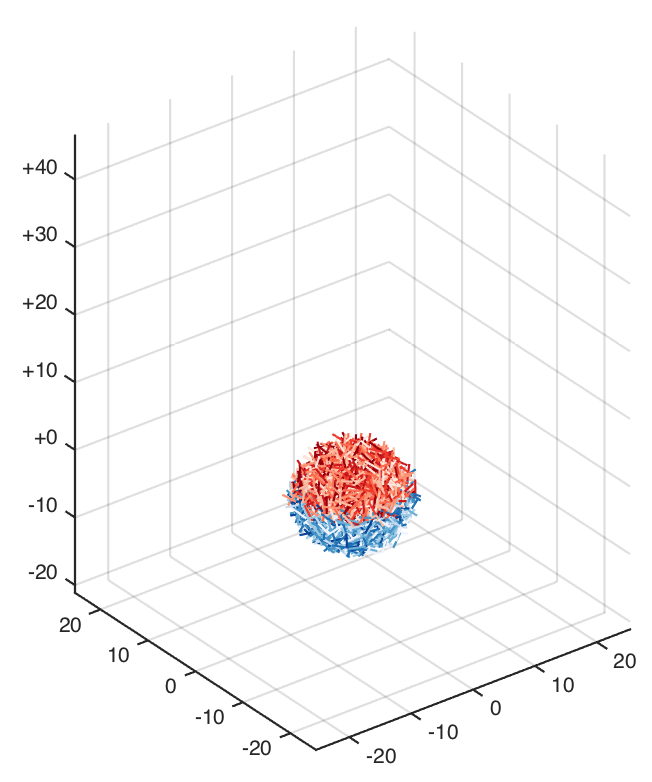
\includegraphics[width=\textwidth]{img/mixing/top_00000.pdf}
    \caption{$t=0$}\label{fig:mixing_top_a}
  \end{subfigure}
  \begin{subfigure}[h]{0.24\textwidth}
    \centering
    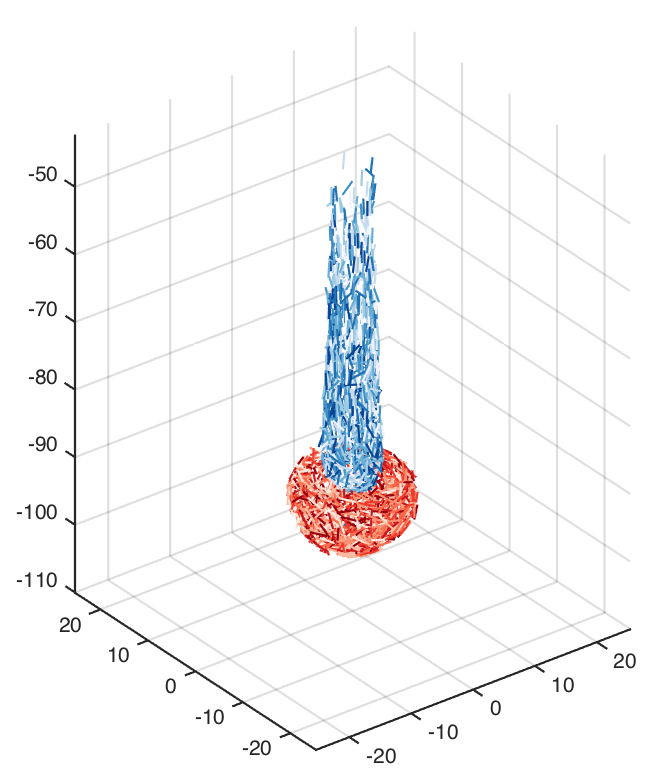
\includegraphics[width=\textwidth]{img/mixing/top_00020.pdf}
    \caption{$t=20$}\label{fig:mixing_top_b}
  \end{subfigure}
  \begin{subfigure}[h]{0.24\textwidth}
    \centering
    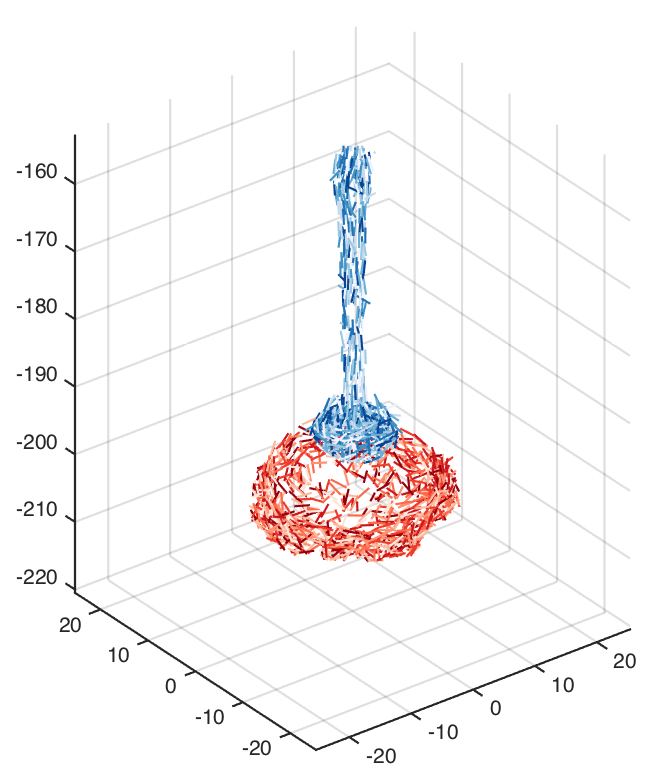
\includegraphics[width=\textwidth]{img/mixing/top_00060.pdf}
    \caption{$t=60$}\label{fig:mixing_top_c}
  \end{subfigure}
  \begin{subfigure}[h]{0.24\textwidth}
    \centering
    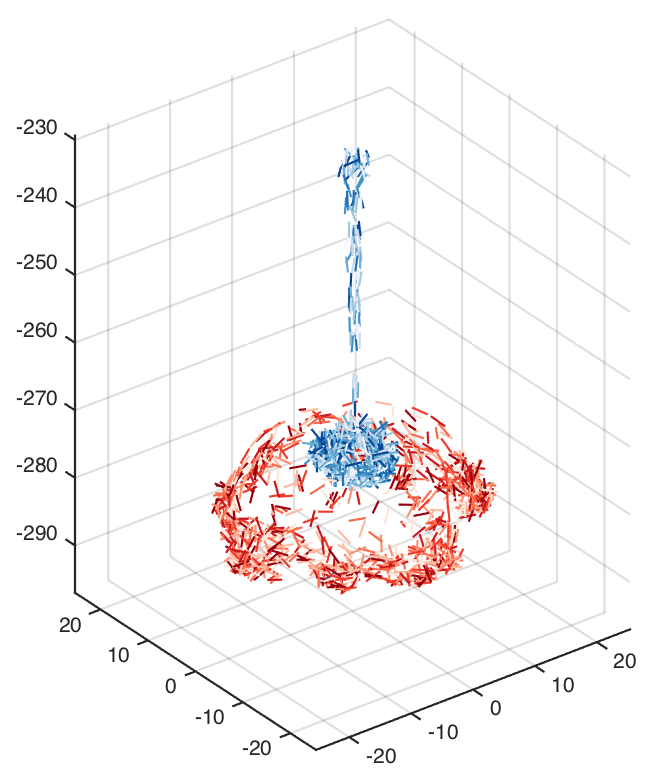
\includegraphics[width=\textwidth]{img/mixing/top_00100.pdf}
    \caption{$t=100$}\label{fig:mixing_top_d}
  \end{subfigure}
  \caption[Unmixed sphere]{Unmixed sphere. Starting the sedimentation with the high density fibers (red) as the top half and the low density fibers (blue) as the bottom half of the sphere.}
  \label{fig:unmixed_sphere}
\end{figure}

In contrast to the configuration with an unmixed sphere, Fig.~\ref{fig:mixed_sphere} shows a similar simulation, starting with a randomly mixed sphere (Fig.~\ref{fig:mixing_random_a}). The beginning of the simulation behaves similar to the unmixed case, but the separation does not happen as fast and far fewer lower density fibers are lost from the sphere (Fig.~\ref{fig:mixing_random_b}). Both the larger higher density and the smaller lower density torus form again. Yet in contrast to the unmixed case both groups stay closer together. The close proximity prevents the groups from completely separating and causes the higher density torus to be sucked down by the passing lower density torus (Fig.~\ref{fig:mixing_random_c}). During the following timesteps the two toruses appear to form an interlocked torus, which continues to sediment  (Fig.~\ref{fig:mixing_random_d}). Eventually the interlocked torus breaks up and fibers scatter. 

\begin{figure}[!htbp]
  \centering
  \begin{subfigure}[h]{0.24\textwidth}
    \centering
    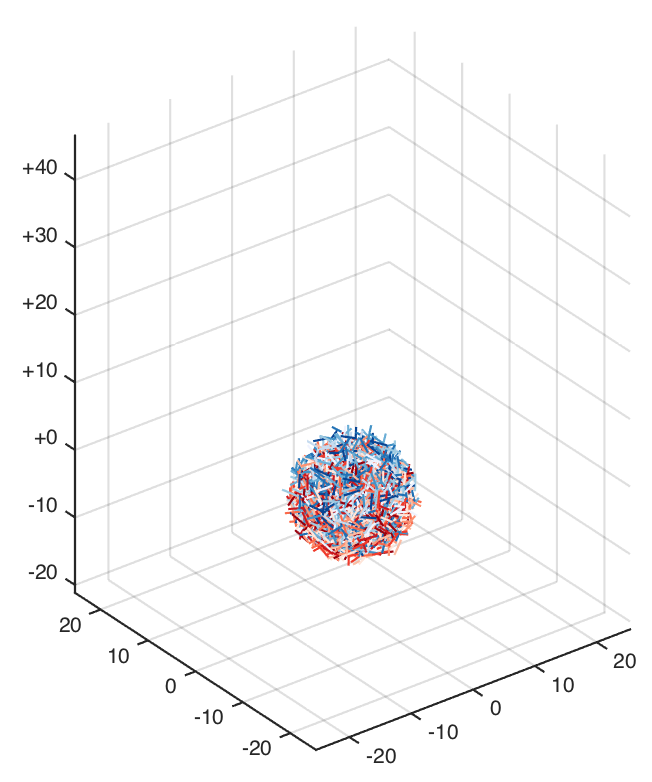
\includegraphics[width=\textwidth]{img/mixing/random_00000.pdf}
    \caption{$t=0$}\label{fig:mixing_random_a}
  \end{subfigure}
  \begin{subfigure}[h]{0.24\textwidth}
    \centering
    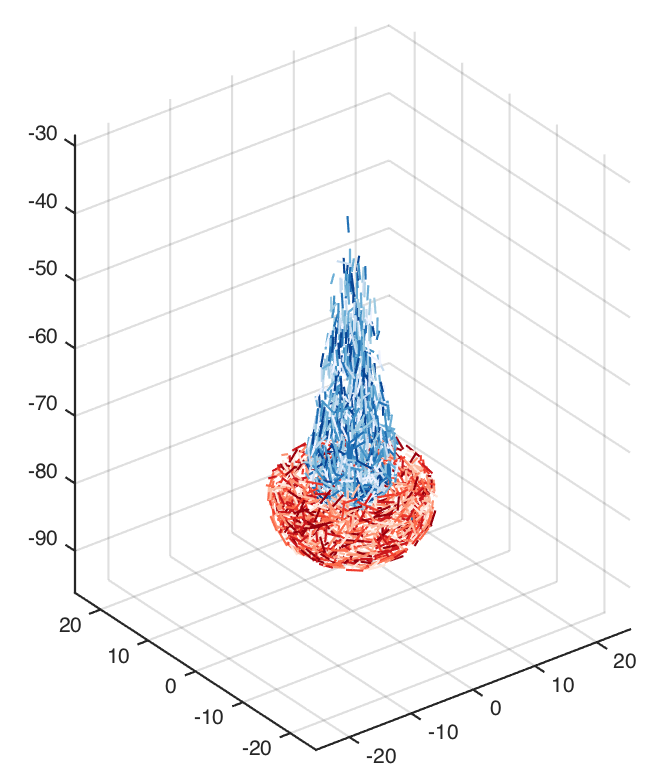
\includegraphics[width=\textwidth]{img/mixing/random_00020.pdf}
    \caption{$t=20$}\label{fig:mixing_random_b}
  \end{subfigure}
  \begin{subfigure}[h]{0.24\textwidth}
    \centering
    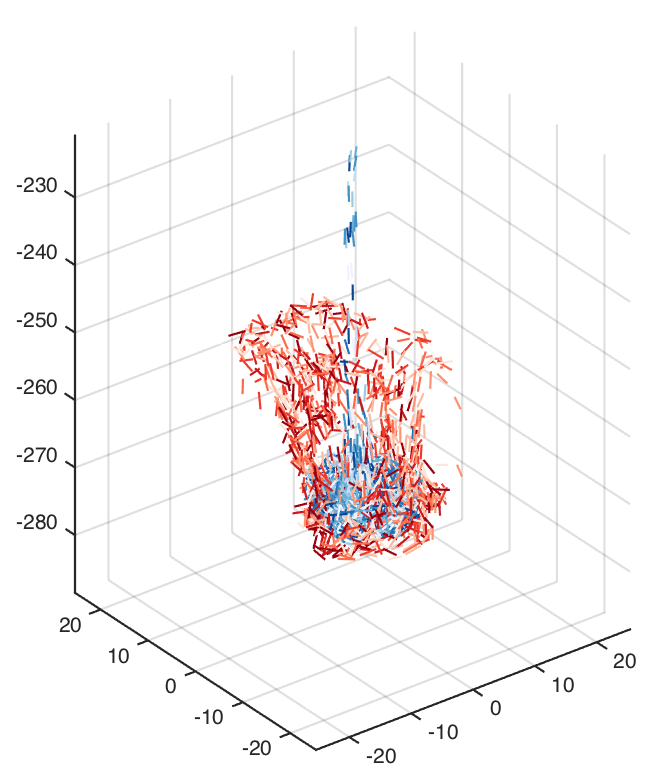
\includegraphics[width=\textwidth]{img/mixing/random_00100.pdf}
    \caption{$t=100$}\label{fig:mixing_random_c}
  \end{subfigure}
  \begin{subfigure}[h]{0.24\textwidth}
    \centering
    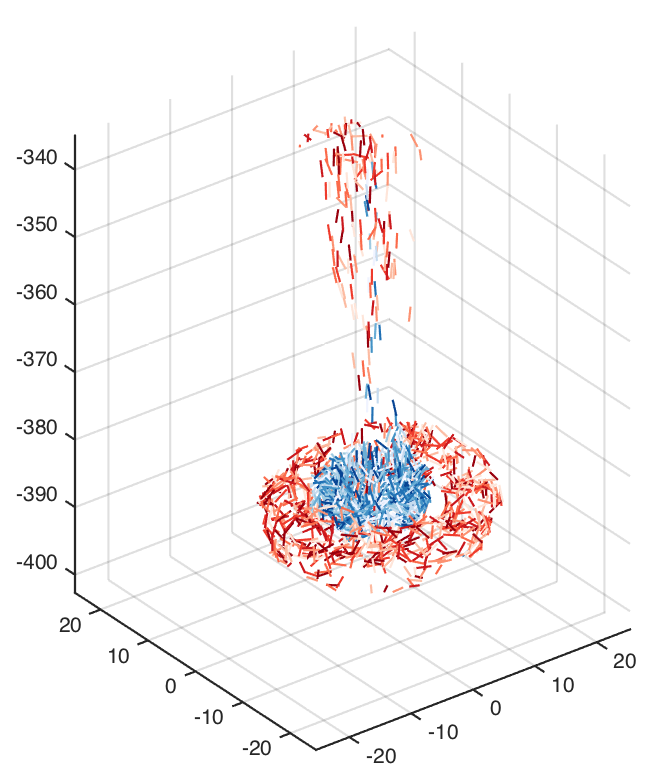
\includegraphics[width=\textwidth]{img/mixing/random_00150.pdf}
    \caption{$t=150$}\label{fig:mixing_random_d}
  \end{subfigure}
  \caption[Mixed sphere]{Mixed sphere. Starting the sedimentation with the high density fibers (red) and the low density fibers (blue) randomly mixed inside the sphere.}
  \label{fig:mixed_sphere}
\end{figure}

The results for the mixed and unmixed sphere with rigid straight fibers do largely agree with the results of spherical particles from Bülow et al.~\cite{Bulow2015}. However, both simulation methods and setups are very different which makes a comparison very challenging. Furthermore our experiment are only a first step and many more experiments have to be cared out to get a deeper understanding of the behavior of rigid fibers in a mixed sphere. Exploring the impact of initial fiber configuration, the density ratio and the fiber concentration are all exciting future research opportunities.
